\documentclass[11pt]{article}

\usepackage[
% fancytheorems, 
% fancyproofs,
noindent, 
nokoma
%spacingfix, 
]{adam}

% \usepackage{ulem}
% \DeclareRobustCommand{\hsout}[1]{\texorpdfstring{\sout{#1}}{#1}}

\usepackage{cancel}
\usepackage{physics}
\usepackage{amsmath}
\usepackage{tikz}
\usepackage{mathdots}
\usepackage{mleftright}
\usepackage{yhmath}
\usepackage{cancel}
\usepackage{color}
\usepackage{siunitx}
\usepackage{array}
\usepackage{multirow}
\usepackage{amssymb}
\usepackage{gensymb}
\usepackage{tabularx}
\usepackage{extarrows}
\usepackage{booktabs}
\usetikzlibrary{fadings}
\usetikzlibrary{patterns}
\usetikzlibrary{shadows.blur}
\usetikzlibrary{shapes}

\makeatletter
\renewcommand*\env@matrix[1][*\c@MaxMatrixCols c]{%
  \hskip -\arraycolsep
  \let\@ifnextchar\new@ifnextchar
  \array{#1}}
\makeatother


% \usepackage{titling}
% \setlength{\droptitle}{-4em}


\title{\vspace{-3\baselineskip}\ \\A Crash Course in Integration in $\R^2$ and $\R^3$}
\author{CircleThm\#7102}
\date{\today}

\begin{document}

\maketitle

This is a no-frills description of how to integrate over curves, areas, volumes and surfaces in $\R^2$ and $\R^3$. Very little will be actually motivated, but it should (hopefully) still be helpful.


\section{The Line Integral}

Suppose you have a regular curve $C$, parametrised by some function $\vv{x}(t)$, where $a \leq t \leq b$, and you want to integrate some other function $f: \R^3 \rightarrow \R$ over the curve. 

\begin{center}
	


	\tikzset{every picture/.style={line width=0.75pt}} %set default line width to 0.75pt        

	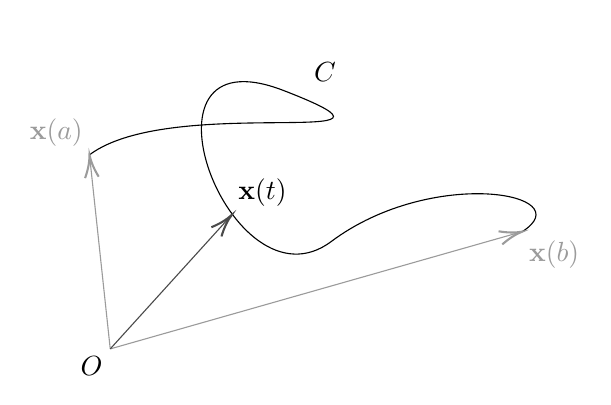
\begin{tikzpicture}[x=0.75pt,y=0.75pt,yscale=-1,xscale=1]
	%uncomment if require: \path (0,300); %set diagram left start at 0, and has height of 300
	
	%Curve Lines [id:da9004923069124608] 
	\draw    (113.5,66.25) .. controls (153.5,36.25) and (284.5,65.25) .. (207,35.25) .. controls (129.5,5.25) and (181.5,144.25) .. (230,108) .. controls (278.5,71.75) and (351,84.75) .. (322,103.25) ;
	%Straight Lines [id:da2156158537362194] 
	\draw [color={rgb, 255:red, 155; green, 155; blue, 155 }  ,draw opacity=1 ]   (123.5,159.75) -- (113.71,68.24) ;
	\draw [shift={(113.5,66.25)}, rotate = 443.9] [color={rgb, 255:red, 155; green, 155; blue, 155 }  ,draw opacity=1 ][line width=0.75]    (10.93,-3.29) .. controls (6.95,-1.4) and (3.31,-0.3) .. (0,0) .. controls (3.31,0.3) and (6.95,1.4) .. (10.93,3.29)   ;
	%Straight Lines [id:da579111129191187] 
	\draw [color={rgb, 255:red, 155; green, 155; blue, 155 }  ,draw opacity=1 ]   (123.5,159.75) -- (320.08,103.8) ;
	\draw [shift={(322,103.25)}, rotate = 524.11] [color={rgb, 255:red, 155; green, 155; blue, 155 }  ,draw opacity=1 ][line width=0.75]    (10.93,-3.29) .. controls (6.95,-1.4) and (3.31,-0.3) .. (0,0) .. controls (3.31,0.3) and (6.95,1.4) .. (10.93,3.29)   ;
	%Straight Lines [id:da9169004089653635] 
	\draw [color={rgb, 255:red, 74; green, 74; blue, 74 }  ,draw opacity=1 ]   (123.5,159.75) -- (180.66,96.73) ;
	\draw [shift={(182,95.25)}, rotate = 492.21] [color={rgb, 255:red, 74; green, 74; blue, 74 }  ,draw opacity=1 ][line width=0.75]    (10.93,-3.29) .. controls (6.95,-1.4) and (3.31,-0.3) .. (0,0) .. controls (3.31,0.3) and (6.95,1.4) .. (10.93,3.29)   ;
	
	% Text Node
	\draw (220.5,20.5) node [anchor=north west][inner sep=0.75pt]    {$C$};
	% Text Node
	\draw (111.5,63.25) node [anchor=south east] [inner sep=0.75pt]  [color={rgb, 255:red, 155; green, 155; blue, 155 }  ,opacity=1 ]  {$\mathbf{x}( a)$};
	% Text Node
	\draw (108,162) node [anchor=north west][inner sep=0.75pt]    {$O$};
	% Text Node
	\draw (324,106.25) node [anchor=north west][inner sep=0.75pt]  [color={rgb, 255:red, 155; green, 155; blue, 155 }  ,opacity=1 ]  {$\mathbf{x}( b)$};
	% Text Node
	\draw (184,92.25) node [anchor=south west] [inner sep=0.75pt]    {$\mathbf{x}( t)$};
	
	
	\end{tikzpicture}
	
\end{center}

Then we have, integrating from $\vv{x}(a)$ to $\vv{x}(b)$,
$$
\int_C f(\vv{x}) \dd s = \int_a^b f(\vv{x}(t)) \left|\frac{\dd \vv x(t)}{\dd t}\right| \dd t.
$$

If instead we wanted to integrate over some vector field (by say taking the dot product of that vector field with the unit tangent), then since $\dd \vv{x}(t) / \dd t$ is tangent to the curve, we would have
$$
\int_C F(\vv{x}) \cdot \dd \vv{x} = \int_a^b \vv{F}(\vv{x}(t)) \cdot \frac{\dd \vv{x}}{\dd t} \dd t,
$$
where again we integrate from $\vv{x}(a)$ to $\vv{x}(b)$.

\section{Area and Volume Integrals}

Suppose you have some closed region $D \subset \R^2$, and you wanted to integrate some function $f: \R^2 \rightarrow \R$ over the region. 

\begin{center}
	

\tikzset{every picture/.style={line width=0.75pt}} %set default line width to 0.75pt        

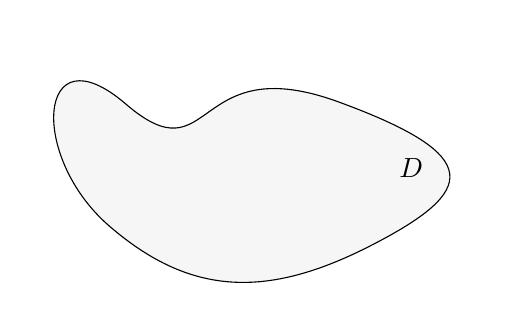
\begin{tikzpicture}[x=0.75pt,y=0.75pt,yscale=-1,xscale=1]
%uncomment if require: \path (0,300); %set diagram left start at 0, and has height of 300

%Shape: Polygon Curved [id:ds07060702255371465] 
\draw  [fill={rgb, 255:red, 246; green, 246; blue, 246 }  ,fill opacity=1 ] (179,76.25) .. controls (221.5,112.75) and (210.5,49.25) .. (281.5,75.25) .. controls (352.5,101.25) and (348,118.25) .. (297.5,144.25) .. controls (247,170.25) and (210,168.75) .. (171,135) .. controls (132,101.25) and (136.5,39.75) .. (179,76.25) -- cycle ;

% Text Node
\draw (309.5,101.5) node [anchor=north west][inner sep=0.75pt]    {$D$};


\end{tikzpicture}

\end{center}

Then integrate over say the $x$ coordinate first (where the bounds of the inner integral will depend on $y$), we have
$$
\int \int_D f(\vv{x}) \dd A = \int \int_{(x, y) \in D} f(x, y) \dd x \; \dd y
$$

Of course we could have integrated over the $y$ coordinate first, and would probably give the same result.

We can also do a change of coordinate. Suppose we have $x = x(u,v)$ and $y = y(u, v)$ being smooth bijections (with smooth inverse) mapping $D'$ in the $(u, v)$-plane to the region $D$ in the $(x, y)$-plane. Then we have
$$
\int \int_{(x, y) \in D} f(x, y) \dd x \; \dd y = \int \int_{(u, v) \in D'} f(x(u, v), y(u, v)) |J| \dd u \; \dd v,
$$
where
% $$
% 	|J| = \left|\frac{\partial (x, y)}{\partial (u, v)}\right| = \left|\det\begin{pmatrix}[c|c]
% 		\dfrac{\partial \vv{x}}{\partial u} & \dfrac{\partial \vv{x}}{\partial v}
% 	  \end{pmatrix}\right|=
% $$
$$
	|J| = \left|\frac{\partial (x, y)}{\partial (u, v)}\right| = \biggl|\det\biggl(
		\frac{\partial \vv{x}}{\partial u} \mathrel{\Big|} \frac{\partial \vv{x}}{\partial v}
	  \biggr)\biggr|=\left|\det\begin{pmatrix}
		\frac{\partial x}{\partial u} & \frac{\partial x}{\partial v} \\
		\frac{\partial y}{\partial u} & \frac{\partial y}{\partial v}
		\end{pmatrix}\right|
$$
is the \emph{Jacobian}.

Basically the exact same thing is true for volume integrals -- I won't bore you with the details. Just use three variables and change the Jacobian accordingly.

\clearpage

\section{Surface Integrals}

Suppose you have a surface $S$, parametrised with
$$
S = \{\vv{x}(u, v) \mid (u, v) \in D\},
$$
for some region $D$ in the ($u$, $v$)-plane. Suppose also that you wanted to integrate some function $f: \R^3 \rightarrow \R$ over the surface.

\begin{center}
	

\tikzset{every picture/.style={line width=0.75pt}} %set default line width to 0.75pt        

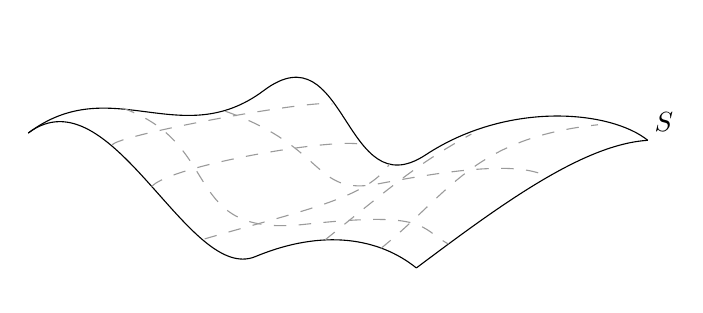
\begin{tikzpicture}[x=0.75pt,y=0.75pt,yscale=-1,xscale=1]
%uncomment if require: \path (0,300); %set diagram left start at 0, and has height of 300

%Curve Lines [id:da8331094955191735] 
\draw    (69.5,148.25) .. controls (109.5,118.25) and (143,157.75) .. (183,127.75) ;
%Curve Lines [id:da02971412381563232] 
\draw    (183,127.75) .. controls (223,97.75) and (221.5,184.75) .. (261,158.75) .. controls (300.5,132.75) and (350,137.25) .. (368,151.75) ;
%Curve Lines [id:da06249824765767975] 
\draw    (256.5,213.25) .. controls (296.5,183.25) and (336.5,153.75) .. (368,151.75) ;
%Curve Lines [id:da5475138078285074] 
\draw    (69.5,148.25) .. controls (109.5,118.25) and (146.5,221.25) .. (179,207.75) .. controls (211.5,194.25) and (238.5,198.75) .. (256.5,213.25) ;
%Curve Lines [id:da749702573016355] 
\draw [color={rgb, 255:red, 155; green, 155; blue, 155 }  ,draw opacity=1 ] [dash pattern={on 4.5pt off 4.5pt}]  (110,154) .. controls (112,149.25) and (207,131.75) .. (216,134.25) ;
%Curve Lines [id:da9289119498181688] 
\draw [color={rgb, 255:red, 155; green, 155; blue, 155 }  ,draw opacity=1 ] [dash pattern={on 4.5pt off 4.5pt}]  (129,174) .. controls (138,163.75) and (222,149.25) .. (232,154.25) ;
%Curve Lines [id:da2876439573644143] 
\draw [color={rgb, 255:red, 155; green, 155; blue, 155 }  ,draw opacity=1 ] [dash pattern={on 4.5pt off 4.5pt}]  (154.5,199.25) .. controls (202.5,185.25) and (232.5,179.75) .. (243.5,163.25) ;
%Curve Lines [id:da3276657339566953] 
\draw [color={rgb, 255:red, 155; green, 155; blue, 155 }  ,draw opacity=1 ] [dash pattern={on 4.5pt off 4.5pt}]  (212.5,199.75) .. controls (246,172.75) and (257.5,162.75) .. (283,148.75) ;
%Curve Lines [id:da5089254389183103] 
\draw [color={rgb, 255:red, 155; green, 155; blue, 155 }  ,draw opacity=1 ] [dash pattern={on 4.5pt off 4.5pt}]  (239.5,203.75) .. controls (273,176.75) and (284,150.75) .. (344,144.25) ;
%Curve Lines [id:da14219428695386094] 
\draw [color={rgb, 255:red, 155; green, 155; blue, 155 }  ,draw opacity=1 ] [dash pattern={on 4.5pt off 4.5pt}]  (115,136.25) .. controls (164.5,153.75) and (142.5,198.75) .. (202.5,192.25) .. controls (262.5,185.75) and (257.5,193.75) .. (272,201.75) ;
%Curve Lines [id:da4864039302311194] 
\draw [color={rgb, 255:red, 155; green, 155; blue, 155 }  ,draw opacity=1 ] [dash pattern={on 4.5pt off 4.5pt}]  (164.5,137.75) .. controls (214,155.25) and (206.5,178.75) .. (238,172.75) .. controls (269.5,166.75) and (305,161.25) .. (319.5,169.25) ;

% Text Node
\draw (370,148.75) node [anchor=south west] [inner sep=0.75pt]    {$S$};


\end{tikzpicture}

\end{center}

Then we would have
$$
\int \int_S f(\vv{x}) \dd S = \int \int_D f(\vv{x}(u, v)) \left|\frac{\partial \vv{x}}{\dd u} \times \frac{\partial \vv{x}}{\partial v}\right| \dd u\; \dd v.
$$
If instead we wanted to integrate over some vector field $\vv{F} : \R^3 \rightarrow \R^3$ by taking the dot product of the vector field with the unit normal (a flux integral), then since $\frac{\partial \vv{x}}{\dd u} \times \frac{\partial \vv{x}}{\partial v}$ is normal to the curve, we would have
$$
\int \int_S \vv{F}(\vv{x}) \cdot \dd \vv{S} = \int \int_D \vv{F}(\vv{x}(u, v)) \cdot \left(\frac{\partial \vv{x}}{\dd u} \times \frac{\partial \vv{x}}{\partial v} \right)\dd u\; \dd v.
$$
It's worth noting here that by doing this, we implicitly chose a direction for the normal (there's 2!). If we wanted the other direction, we can just negate the integral. 
\clearpage
\section{Integral Theorems}

Having read that, you are clearly now an expert integrator, keen to speed up your multidimensional calculations. Luckily we have a few results at our disposal which we will state (naturally) without proof. Throughout, we will use the notation $\partial A$ to denote the boundary of $A$.

\begin{theorem}[Conservative Vector Fields]
	Suppose the vector field $\vv{F}$ can be written as $\vv{F} = \nabla f$ for some scalar function $f$. Then if $C$ is any curve from $\vv{x}(a)$ to $\vv{x}(b)$, we have
	$$
	\int_C \vv{F} \cdot \dd \vv{x} = f(\vv{x}(b)) - f(\vv{x}(a)).
	$$
\end{theorem}

\begin{theorem}[Green's Theorem]
	$P=P(x, y)$ and $Q=Q(x, y)$ are continuously differentiable functions on $A$ and $\partial A$ is made from a collection of piecewise smooth curves, then
$$
\int_{\partial A} P \mathrm{~d} x+Q \mathrm{~d} y=\iint_{A}\left(\frac{\partial Q}{\partial x}-\frac{\partial P}{\partial y}\right) \mathrm{d} x \mathrm{~d} y .
$$
The orientation of the boundary $\partial A$ is such that A lies to your left as you traverse it.
\end{theorem}

\begin{theorem}[Stokes' Theorem]
If $\mathbf{F}=\mathbf{F}(\mathbf{x})$ is a continuously differentiable vector field and $S$ is an orientable, piecewise regular surface with piecewise regular boundary $\partial S$ then
$$
\int_{S}(\nabla \times \mathbf{F}) \cdot \mathrm{d} \mathbf{S}=\int_{\partial S} \mathbf{F} \cdot \mathrm{d} \mathbf{x}.
$$
\end{theorem}

\begin{theorem}[Divergence Theorem in $\R^3$]
	If $\mathbf{F}=\mathbf{F}(\mathbf{x})$ be a continuously differentiable vector field and $V$ is a volume with a piecewise regular boundary $\partial V$ then
$$
\int_{V} \nabla \cdot \mathbf{F}\; \mathrm{d} V=\int_{\partial V} \mathbf{F} \cdot \mathrm{d} \mathbf{S}
$$
where the normal to $\partial V$ points outwards from $V$.
\end{theorem}

\begin{theorem}[Divergence Theorem in $\R^2$]
	Let $\mathbf{F}=\mathbf{F}(\mathbf{x})$ be a continuously differentiable vector field and $D \subset \R^{2}$ region with piecewise smooth boundary $\partial D$ then
	$$
	\int_{D} \nabla \cdot \mathbf{F} \;\mathrm{d} A=\oint_{\partial D} \mathbf{F} \cdot \mathbf{n} \mathrm{d} s
	$$
	where the unit normal $\vv{n}$ to $\partial D$ points outwards from $D .$
\end{theorem}


\end{document}
